\chapter{Experimental Results}
% Presentation of results
% Detailed analysis of results
The goal of this chapter is to discuss the experimental results obtained by the proposed algorithm using the evaluation methods  presented in  Chapter 5, as well as the results obtainned from intermediate steps such as Pre-Processing and Parameter Optimisation. 

The input data used for the experiments are the two meeting transcripts IB4010 and IS1008c with the BET questions for these meetings as described in Chapter 3. In addition to the experimental data, automated transcripts generated by the Automatic Speech Recognition, namely ASR transcripts and some automatic summaries based on ASR transcripts are also used. 

Because that two meetings may have different difficulties, we analyzed the results for each meeting separately.

\section{Data Processing}


First of all, we present the result for the pre-processing stage, questions and transcript are processed by removing unuseful information as punctuation marks, stopwords and pronominal words and being transformed into a standard form to enhance the performance of lexical similarity algorithm as described in the Section 4.1.

After removing the stopwords (see Appendix for the full list of stopwords), the length of IB4010 is 4872 words compared to 9488 words in the original transcript. After the same processing, the length of IS1008c is 2059 words compared to 4000 words in the original transcript. This means that nearly half of the total amount of words are removed. This helps because it doubles the algorithm speed when it searches relevant passages in the transcript.

For the questions, after the pre-processing, the average length of the questions is 8 words compared to 12 words in original questions. Reducing the length of the questions also plays an important role in speeding up the algorithm, because it is used as the base unit to define size of the parameters for a search window (see the definition of search window in the section 4.2).

\section{System Performance}


This section shows the results of the algorithm for both IB4010 and IS1008c using the evaluation methods presented in the Chapter 5.

The experimental results show the performance of both principal phases of the algorithm, Passage Retrieval and True-False Answer. The contribution of each technique in the algorithm such as n-gram matching and speaker-directed scores assigned to matched words are also demonstrated by showing obtainned scores for each technique separately. 

In order to show the effectiveness of the algorithm, the scores obtained by guessing the answers randomly, which is also calculated and compared with the results of the algorithm. The \textit{random} scores for true-false answers are 50\% because there are only two values \textit{True} or \textit{False} for an answer. The \textit{random} scores for passage retrieval are calculated as follows:

With a defined search window and input data, we can compute the total of possible passages in the transcript based on transcript size, search window size and search window step. The search window moves on through the transcript from one place to another. At one time, the position of the window defines a passage that has the same position and same size as the window. Thus, the number of window movements is the total number of passages. The distance of two consecutive positions of the search window movement is defined as the \textit{step} of search window. Consequently, the total passages is calculated as in the Equation \ref{equation: number_passage}.
  \begin{equation}
\label{equation: number_passage}
	Total \; Passages = [(transcript \; size - window \; size)/window \; step] + 1
\end{equation}
   If a candidate passage and corresponding reference passage overlap each other by one word, the candidate passage is considered to be true and the average of reference passage is 10 words, we have total number of correct passages \textit{10 \ensuremath{\times} (window size / window step)}. Therefore, \textit{random} score is calculated by dividing the number of correct passages by the total number of passages. In the section 6.1, we have the average of question size is 8 words, the length of transcript IB4010 is 4872 and the length of transcript IS1008c. From this numbers, calculated \textit{random} score for IB4010 is 1.65\% and for IS1008c is 3.9\%.

%Correct passage = 2*(window size / window step)
%
%Random score = correct passage/(total passages)
%
%\ensuremath{\Rightarrow} IB4010 score = (2*8*7/7) / ([(4872 - 8*7)/7)   = 0.33%
%
%\ensuremath{\Rightarrow} IS1008c score = (2*8*7/7) / ([(2059 - 8*7)/7)   =  0.78%

% Yes, explain a bit more

The method of Cross-Validation is used to calculate the average of scores as described in the pseudo codes \ref{alg: Cross-Validation}.





Results for the two processing stages of the automatic BET question answering algorithm are given in the Table \ref{Performance of the algorithm over two meetings}, for three variants of the algorithm: using only unigram matching when computing the similarity score (and no weighting of speaker-specific words), then with N-gram matching, and finally with additional weighting of matched words spoken by a speaker mentioned in the question, as explained in the Chapter 4.2.

Passage retrieval provides excellent results compared with the chances of randomly locating the correct passage, with scores of 0.55 \ensuremath{\pm} 0.14 for IB4010 and 0.62 \ensuremath{\pm} 0.16 for IS1008c (obtained with 5-fold cross validation) compared with 1.65\% and 3.9\% respectively for the \textit{random} score values. The automatic system is of course much faster than humans+browsers, at less than 1s per question.

When combined with the question discrimination, the performance increases only slightly. The expected score should be an average of the score on the questions for which the passage was correctly identified (55\% and 62\%) with a 50\%  chance for the questions on which the passage was incorrectly identified, so about (55+22=77)\% for IB4010 and (62+19=81)\% for IS1008c. 

The fact that the actual scores are lower (though above chance) shows that the algorithm needs improvement for this stage.


\begin{table}[htbp]
\caption{Performance of the algorithm over two meetings}
\begin{center}
\begin{tabular}{|l|l|l|l|l|l|l|l|l|}
\hline
\multicolumn{ 1}{|c|}{\textbf{Condition}} & \multicolumn{ 4}{c|}{\textbf{Passage Retrieval}} & \multicolumn{ 4}{c|}{\textbf{True-False Answer}} \\ \cline{ 2- 9}
\multicolumn{ 1}{|c|}{} & \multicolumn{ 2}{c|}{\textbf{IB4010}} & \multicolumn{ 2}{c|}{\textbf{IS1008c}} & \multicolumn{ 2}{c|}{\textbf{IB4010}} & \multicolumn{ 2}{c|}{\textbf{IS1008c}} \\ \cline{ 2- 9}
\multicolumn{ 1}{|c|}{} & \multicolumn{1}{c|}{\textbf{Acc.}} & \multicolumn{1}{c|}{\textbf{Stdev}} & \multicolumn{1}{c|}{\textbf{Acc.}} & \multicolumn{1}{c|}{\textbf{Stdev}} & \multicolumn{1}{c|}{\textbf{Acc.}} & \multicolumn{1}{c|}{\textbf{Stdev}} & \multicolumn{1}{c|}{\textbf{Acc.}} & \multicolumn{1}{c|}{\textbf{Stdev}} \\ \hline
Random & 0.017 & n/a & 0.039 & n/a & 0.50 & n/a & 0.50 & n/a \\ \hline
Unigram matching & 0.27 & 0.15 & 0.54 & 0.21 & 0.37 & 0.14 & 0.36 & 0.21 \\ \hline
N-gram matching & 0.32 & 0.15 & 0.50 & 0.19 & 0.43 & 0.17 & 0.42 & 0.11 \\ \hline
N-gram + speaker & 0.55 & 0.14 & 0.62 & 0.16 & 0.57 & 0.06 & 0.64 & 0.18 \\ \hline
\end{tabular}
\end{center}
\label{Performance of the algorithm over two meetings}
\end{table}


The standard deviation is calculated based on results from the Cross-Validation method using the formula \ref{equation: standard deviation}.

One remark is here that the true-false answer stage use the results of the passage retrieval stage as input data. If the results of the first stage are not good, the second stage can not give the nice results. This is why, in the table \ref{Performance of the algorithm over two meetings} the results of the single 1-gram matching or single n-gram matching is even worse than the random results for the true-false answers.



Our proposed algorithm, based on the algorithm of lexical similarity using n-gram matching and speaker-directed scores assigned to matched words in the passage retrieval  \cite{lequocanh1}, demonstrates the effectiveness of these techniques by the results displayed in the table. Despite the simplicity of the second phase of the algorithm, its final scores are still significantly above \textit{random} scores.

\section{Experiments with ASR transcripts}

In this section, the performance of the system will be evaluated on ASR transcripts that are generated by an automatic speech recognition. In this case, two ASR transcripts are generated by using the M4 recognition system developed by Karafiat et al \cite{ASR_transcrips}. We will evaluate the obtained results using the ASR transcripts by comparing them with those using the manual transcripts.

According to the report of Karafiat, the quality  of these transcripts are not very good. Logically, scores obtainned over the ASR transcripts should be worse than those over the manual transcripts. The experimental results obtainned by our algorithm using the ASR transcripts as described in the table \ref{results for ASR transcripts} show that the results are good as well. First, the remaining number of words in the ASR transcripts are not much changed compared with those of the manual transcripts. Secondly, although the rate of correct answers over the ASR transcripts decreases as expected, the reduction is only about 8\% compared with the manual transcripts for both phases of the algorithm. This may be explained by the fact that when word error rate of the ASR transcripts affects overall text of the transcripts so that the score of all passages reduces together. The algorithm always chooses the passage of highest score for its answer, thus the accuracy is not much changed. That means the algorithm works robustly when using the ASR transcripts. This is a promising results for building a full automatic assistant tools over ASR meeting transcrips. 

For IB4010, passage retrieval accuracy drops to 0.46 \ensuremath{\pm} 0.13 (from 0.55 \ensuremath{\pm} 0.14) and true-false question accuracy drops to 0.52 \ensuremath{\pm} 0.09 (from 0.57 \ensuremath{\pm} 0.06). For IS1008c, passage retrieval drops to 0.60 \ensuremath{\pm} 0.33 (from 0.62 \ensuremath{\pm} 0.16) and true-false question drops to 0.56 \ensuremath{\pm} 0.19 (from 0.64 \ensuremath{\pm} 0.18).

The two following tables present the results in detail. The method of 5-fold Cross-Validation as described in the Section 5.3 is applied to get the average results over two ASR transcripts. The standard deviations are also calculated according to the formula \ref{equation: standard deviation}.

\begin{table}[htbp]
\caption{Experimental results for ASR transcripts}
\begin{tabular}{|l|c|c|c|c|}
\hline
\multicolumn{1}{|c|}{} & \multicolumn{ 2}{c|}{IB4010 transcript} & \multicolumn{ 2}{c|}{IS1008c transcript} \\ \hline
\multicolumn{1}{|c|}{} & Manual & ASR & Manual & ASR \\ \hline
Original length & 9488 & 9393 & 4000 & 3927 \\ \hline
Processed length & 4872 & 4624 & 2059 & 1957 \\ \hline
Passage retrieval & 55\%\ensuremath{\pm}14\% & 46\%\ensuremath{\pm}13\% & 62\%\ensuremath{\pm}16\% & 60\%\ensuremath{\pm}34\% \\ \hline
True-false answer & 57\%\ensuremath{\pm}6\% & 52\%\ensuremath{\pm}9\% & 64\%\ensuremath{\pm}18\% & 56\%\ensuremath{\pm}19\% \\ \hline
\end{tabular}
\label{results for ASR transcripts}
\end{table}


%%%%%%%%%%%%%%%%%%%%%%%%%%%%%%%%%%%%%%%%%%%%

\section{Summarization Results}

A meeting transcript summary is a transcript that is shorter than the original, but on that still contains the main information of the meeting.

In this section, the system is tested on summaries of two meeting transcripts IB4010 and IS1008c based on ASR transcripts, named ASR summaries. There are two purposes for this test. First, it aims to measure the quality of an ASR summary by its scores when it is used to replace the original transcript. Secondly, it helps to evaluate the robustness of proposed algorithm, which should give a number of correct answers that decreases little by little when the length of summaries reduces, because some important information is lost from the processing of the ASR.

For an evaluation purpose, for each ASR summary, we generate a corresponding \textit{random} summary in order to compare scores of ASR summaries with those of random summaries. This helps us to evaluate indirectly the summarization method as well. If the summarization algorithm is good, the score schema of its summaries must be different from that of the random summaries. A random summary is created by repeating the elimination of a transcript word randomly until this summary has the same length of the ASR summary. In order to increase the precision of the results over random summaries, for each known summary length, we create 100 random summaries and calculate their average scores.

The ASR summaries used in these experiments were created by an automatic summarization system presented by Gabriel Murray and Steve Renals \cite{ASR_summaries} using term-weights. Within these, each dialogue act is ranked by a score of importance level, namely ranking score. Based on these ranking scores, we create different summaries by eliminating utterances whose ranking score is less than a defined threshold.

In reality, we define 10 different thresholds. The obtained results are displayed in two tables \ref{tab: Results for IS1008c summaries} and \ref{tab: Results for IB4010 summaries} for IS1008c and IB4010. In the tables, the first column is the percentage of summary length compared with the length of the original transcript. The second column is the threshold, which is used to created a corresponding summary by eliminating all of the utterances whose score is less than this threshold in the transcript. The scores were assigned to each utterance in the transcript by an automatic summarization. When threshold is zero in the first row, the results are presented for original transcript. The four remaining columns are percentages of correct passages and true-false answers for ASR summaries and random summaries, respectively. 

The experimental results lead to the following conclusions:

\begin{itemize}
\item {The number of correct passages for ASR summaries decreases linearly and more quickly than random summaries do when the number of utterances removed from the summaries increases. The graph of summary lengths and the number of correct passages for ASR summaries have the same bias (ie, they are parallel with each other). This says that eliminated utterances for ASR summaries contain important information. This is contrary to the rule of an automatic summarizer that have to remove firstly utterances whose information is less important. The random summaries are even better than the ASR summaries according to the results of correct passages. For evaluation of the algorithm performance, our algorithm works well, in that the number of correct passages decreases linearly for both type of summaries. }
\item {For true-false answers, both type of summaries have the same behaviour. The number of true-false answers decreases logically at first. After that it does not decrease but it tends to a random result. That means the proportion of the correct answers is always around 50\%, meanwhile we know that the probability of a correct true-false answer by chance is also 50\%. This is explained by a fact that true-false answers were answered by the algorithm based on a comparison between two similarity levels, which are obtained by considering each question and its corresponding passage retrieved from the phase Passage Retrieval of the algorithm. At first, decreasing transcript size affects both both true and false question in a pair, the score of corresponding passages decreases accordingly so that the number of correct answers decreases. However, after that, when the important information related to the questions was removed from the transcript due to the automatic summarization, there were not enough facts to distinguish one question from another or in other words, returned answer tends to be random. This demonstrates that the results from the phase True-false Answer are not suitable for aiming to measure the quality of a summary.}

\end{itemize}

Consequently, in this case, the way to eliminate dialogue acts in order to generate a ASR summary did not work very well because it eliminated some important utterances that are necessary to answer the BET questions. In fact, the automatic summarization used to produce the ASR summaries is still experimental and has not seen fully verified. So, the results are only used to evaluate the stability of our system: its performance for the passage retrieval stage is stable over all summaries. Thus, it is promising to be able to use this way to measure the quality of a summary. 




\begin{table}[ht!]
 \scriptsize
\caption{Results for IS1008c summaries (Original length of ASR transcript is 1957 words. The first column presents the percentage of summary length (in comparing with the original transcript) after removing phrases whose score is less than rank score. The second column presents the rank score. The other columns present the percentage of correct answers for passage retrieval and true-false answer.)}
\label{tab: Results for IS1008c summaries}
\begin{tabular}{|c|c|c|c|c|c|}
\hline
\multicolumn{ 1}{|c|}{\%Original Length \tnote{*}} & \multicolumn{ 3}{c|}{ASR Summaries} & \multicolumn{ 2}{c|}{Random Summaries} \\ \cline{ 2- 6}
\multicolumn{ 1}{|c|}{} & rank score & \%cpassage & \%canswer & \%cpassage & \%canswer \\ \hline
100 & \ensuremath{\geq0.00} & 68 & 64 & 68 & 64 \\ \hline
85 & \ensuremath{\geq0.05} & 62 & 62 & 60 & 60 \\ \hline
74 & \ensuremath{\geq0.10} & 56 & 54 & 58 & 60 \\ \hline
64 & \ensuremath{\geq0.15} & 52 & 52 & 54 & 58 \\ \hline
57 & \ensuremath{\geq0.20} & 50 & 48 & 50 & 56 \\ \hline
54 & \ensuremath{\geq0.25} & 46 & 48 & 50 & 56 \\ \hline
52 & \ensuremath{\geq0.30} & 38 & 46 & 50 & 54 \\ \hline
49 & \ensuremath{\geq0.35} & 36 & 46 & 50 & 56 \\ \hline
45 & \ensuremath{\geq0.40} & 28 & 48 & 48 & 52 \\ \hline
41 & \ensuremath{\geq0.45} & 24 & 46 & 46 & 52 \\ \hline
38 & \ensuremath{\geq0.50} & 24 & 46 & 46 & 50 \\ \hline
\end{tabular}
%\begin{tablenotes}
%\item[*] Original length of ASR transcript for IS1008c is 1957 words 
%\end{tablenotes}
\end{table}


%\begin{figure}[hb!]
%\centering
%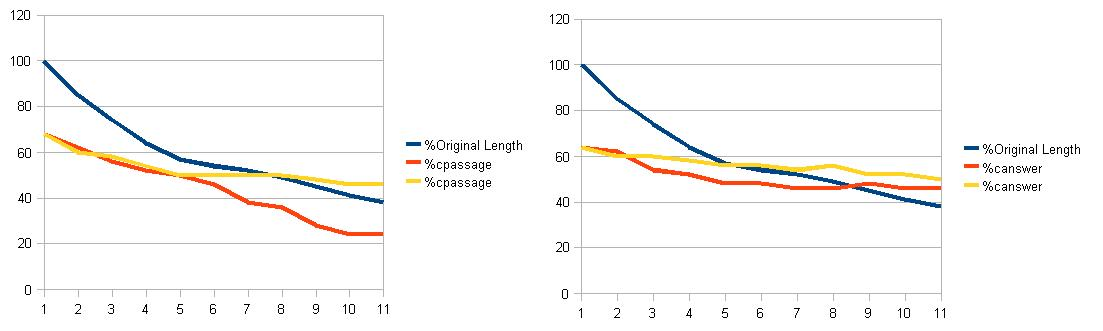
\includegraphics[scale = 0.57]{IS1008c_summaries.jpg}
%\caption{Schemas for IS1008c summaries}
%\label{schema: Results for IS1008c summaries}
%\end{figure}

\begin{table}[hb!]
 \scriptsize
\caption{Results for IB4010 summaries (Original length of ASR transcript is 4624 words. The first column presents the percentage of summary length (in comparing with the original transcript) after removing phrases whose score is less than rank score. The second column presents the rank score. The other columns present the percentage of correct answers for passage retrieval and true-false answer.)}
\begin{tabular}{|c|c|c|c|c|c|}
\hline
\multicolumn{ 1}{|c|}{\%Original Length \tnote{*}} & \multicolumn{ 3}{c|}{ASR Summaries} & \multicolumn{ 2}{c|}{Random Summaries} \\ \cline{ 2- 6}
\multicolumn{ 1}{|c|}{} & rank score & \%cpassage & \%canswer & \%cpassage & \%canswer \\ \hline
100 & \ensuremath{\geq0.00} & 45 & 62 & 45 & 62 \\ \hline
85 & \ensuremath{\geq0.05} & 34 & 51 & 44 & 59 \\ \hline
74 & \ensuremath{\geq0.10} & 26 & 55 & 38 & 56 \\ \hline
65 & \ensuremath{\geq0.15} & 21 & 52 & 37 & 56 \\ \hline
58 & \ensuremath{\geq0.20} & 21 & 54 & 37 & 56 \\ \hline
54 & \ensuremath{\geq0.25} & 20 & 52 & 36 & 56 \\ \hline
51 & \ensuremath{\geq0.30} & 17 & 53 & 36 & 54 \\ \hline
47 & \ensuremath{\geq0.35} & 17 & 53 & 36 & 55 \\ \hline
44 & \ensuremath{\geq0.40} & 16 & 52 & 33 & 54 \\ \hline
40 & \ensuremath{\geq0.45} & 14 & 50 & 35 & 52 \\ \hline
36 & \ensuremath{\geq0.50} & 15 & 51 & 33 & 52 \\ \hline
\end{tabular}
%\begin{tablenotes}
%\item[*] Original length of ASR transcript for IB4010 is 4624 words 
%\end{tablenotes}
\label{tab: Results for IB4010 summaries}
\end{table}


%\begin{figure}[hb!]
%\centering
%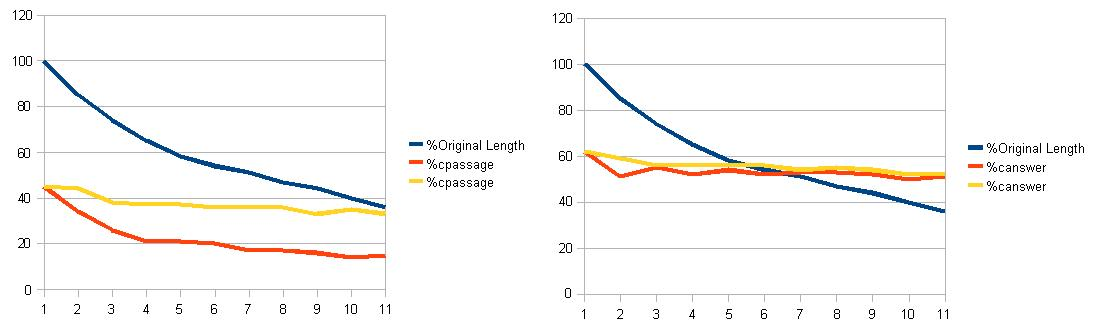
\includegraphics[scale = 0.57]{IB4010_summaries.jpg}
%\caption{Schemas for IB4010 summaries}
%\label{schema: Schemas for IB4010 summaries}
%\end{figure}


\normalsize


\section{Parameter Optimization}

The task of the parameter optimisation is to find the values for the parameters of the algorithm which are best fit for each transcript, IB4010 and IS1008c. The parameters are the search window size and search window step as a proportion of the size of the question. 

In order to do this, we used the 5-fold cross-validation method as presented in the previous chapter to build a statistic table. This table consists of columns and rows which present values of window step and values of window size correspondingly. For instance, for position (2,5), the step of search window is 2 x input question size and the size is 5 x input question size. In this table, each position (row,column) of the table presents the number of partitions as training data of the Cross-Validation method that obtain maximal scores using the value of parameters corresponding to row and column of this position. For instance, the first partition obtains maximal scores at (2,3), (2,5) and the second partition obtain maximal score at (2,4), (2,5) and the others partitions obtain maximal scores at other pairs of parameters, then value of the position (2,5) of the table is 2 corresponding to two partitions. That means when search window size is 2 and search window is 5, there are two partitions over all five partitions obtain maximal score. The maximal scores are the maximal number of true passages retrieved by the algorithm in the first phase. For this experiment, we only use the first phase Passage Retrieval because it is the most essential of the proposed algorithm.

The following tables present results obtained for IB4010 and IS1008c in detail:


 \scriptsize
\begin{center}
\begin{threeparttable}
\caption{Parameter Optimization for IB4010}
\begin{tabular}{|>{\bf}c|c|c|c|c|c|c|c|c|c|c|c|c|c|}
\hline \backslashbox{Size}{Step} & \bf{1} & \bf{2} & \bf{3} & \bf{4} & \bf{5} & \bf{6} & \bf{7} & \bf{8} & \bf{9} & \bf{10} & \bf{11} & \bf{12} & \bf{13} \\ 
\hline 1 &  &  &  &  &  &  &  &  &  &  &  &  &  \\ 
\hline 2 &  &  &  &  &  &  &  &  &  &  &  &  &  \\ 
\hline 3 &  &  &  &  &  &  &  &  &  &  &  &  &  \\ 
\hline 4 &  &  &  &  &  &  &  &  &  &  &  &  &  \\ 
\hline 5 &  &  &  &  &  &  &  &  &  &  &  &  &  \\ 
\hline 6 &  &  &  &  &  &  &  &  &  &  &  &  &  \\ 
\hline 7 &  &  &  &  &  &  &  &  &  &  &  &  &  \\ 
\hline 8 & 1 &  &  & 1 &  &  &  &  &  &  &  &  &  \\ 
\hline 9 & 4 & 3 &  &  &  &  &  &  &  &  &  &  &  \\ 
\hline 10 & 4 & 2 &	\multicolumn{1}{>{\columncolor{yellow}}c}{5}\tnote{*} &  &  &  &  &  &  &  &  &  &  \\ 
\hline 11 & 3 & 2 & 5 &  &  &  &  &  &  &  &  &  &  \\ 
\hline 12 & 1 &  &  &  &  &  &  &  &  &  &  &  &  \\ 
\hline 13 &  & 1 & 2 &  &  &  &  &  &  &  & 1 &  &  \\ 
\hline 
\end{tabular}
\begin{tablenotes}
\item[*] This position is chosen
\end{tablenotes}
\end{threeparttable}
\end{center}



\begin{center}
\begin{threeparttable}
\caption{Parameter Optimization for IS1008c}
%\begin{tabular}{|>{\bf}c|>{\sc}c|}
\begin{tabular}{|>{\bf}c|c|c|c|c|c|c|c|c|c|c|c|c|c|}
\hline \backslashbox{Size}{Step}  & \bf{1} & \bf{2} & \bf{3} & \bf{4} & \bf{5} & \bf{6} & \bf{7} & \bf{8} & \bf{9} & \bf{10} & \bf{11} & \bf{12} & \bf{13} \\ 
\hline 1 &  &  &  &  &  &  &  &  &  &  &  &  &  \\ 
\hline 2 & 1 &  &  &  &  &  &  &  &  &  &  &  &  \\ 
\hline 3 & 1 & 1 & 1 &  &  &  &  &  &  &  &  &  &  \\ 
\hline 4 & \multicolumn{1}{>{\columncolor{yellow}}c}{4}\tnote{*} & 1 & 1 & 1 &  &  &  &  &  &  &  &  &  \\ 
\hline 5 &  &  & 1 & 1 &  &  &  &  &  &  &  &  &  \\ 
\hline 6 & 2 & 2 & 3 & 1 & 2 & 1 &  &  &  &  &  &  &  \\ 
\hline 7 & 1 &  & 3 &  & 2 & 1 &  &  &  &  &  &  &  \\ 
\hline 8 &  &  &  &  &  &  &  & 2 &  &  &  &  &  \\ 
\hline 9 & 3 & 1 & 1 & 1 & 1 & 1 &  &  &  &  &  &  &  \\ 
\hline 10 & 2 &   &	1 & 1 & 1 & 1 &  &  &  & 1 &  &  &  \\ 
\hline 11 & 1 & 1 &   &  &   & 1 & 1 &  &  & 1 &  &  &  \\ 
\hline 12 & 5 & 3 & 3 &  & 2 & 4 & 3 &  &  & 1 & 1 &  &  \\ 
\hline 13 & 1 & 2 & 3 &  & 3 &   & 1 &  &  & 1 & 1 &  &  \\ 
\hline 
\end{tabular}
\begin{tablenotes}
\item[*] This position is chosen 
\end{tablenotes}
\end{threeparttable}
\end{center}

\normalsize 

According to the way of building the table above, parameters are considered good if they help as many training data as possible obtain the maximal scores. Therefore, we will choose parameters at a position whose value is the largest in the table as the relevant parameters. As seen in the table, for IB4010 there are two maximal values at (10,3) and (11,3) and for IS1008c the value of position (12,1) is the largest. These values of parameters are considered to help algorithm obtain the best scores on the training data. However, it is evident that the more the size of a search window increases, the higher the probability that a passage becomes correct. When the size of search window is equal to the size of the transcript, then it certainly contains the information of the question, so the returned \textit{passage} (i.e. the whole meeting) always correct. In this task, we want to find parameters that help program obtain the maximal number of correct passages but the actual objective of the passage retrieval is also to decrease the search space. For this reason, we should choose the smallest size of search window that is suitable for the most partitions. That is why in the table of IS1008c, the position (4,1) is chosen. This means that the size of the search window is 4 times the question size and the step of the search window is 1 time the question size, and are thus the best fit for the BET questions and the transcript IS1008c. 
In the table of IB4010, the pair of parameters (10,3) has the best value, thus the size of search window is 10 and the step of search window is 3 and these are chosen as the best fit for the BET question and the transcript IB4010.

The chosen parameters will be used in the next section.




\section{Comparison with BET scores obtained by human subjects}

 The main goal of this comparison is to discover whether automatic machine and human subjects have the same difficulties in answering the BET questions. By analyzing the scores obtained by the system and by humans, we can also identify in which case this system is useful to help humans answer the BET questions. 

The BET scores used for this comparison are results from BET for the TQB interface \cite{popescubelis2007otm} known as a Transcript-based Query and Browsing Interface. TQB is a meeting browser tool for searching and browsing multi-modal recordings of group meetings. The BET method is used to evaluate the performance of human subjects using this meeting browser over two meetings, IB4010 and IS1008c.

According to the BET method, human subjects that had not worked with TQB before were tested by answering the BET questions using TQB. They were 28 students at the University of Geneva, mainly form the School of Translation and Interpreting. Half of the subjects started with IB4010 and continued with IS1008c, and the other half did the reverse order, thus allowing for differentiated results depending on whether a meeting was seen first or second. That means when subjects worked on the first meeting, they were trained with the TQB interface, so that they answer BET questions were expected to better on the second meeting. And, indeed, the average of precision is a higher for the second meeting. In this experiment, both BET scores of the first meeting and the second meeting are used for comparison with the results obtained by the system. However, the first only 8 BET questions for each meeting are used for this comparison.  We are interested in only two pieces of information from the BET scores: average answering time and precision of each answer. 

In order to set up the configuration of the system, the parameters of search window are used from the previous section Parameter Optimisation. Two pairs (10,3) and (4,1) for IB4010 and IS1008c respectively will be used. That means the size of search window is \textit{10 \ensuremath{\times}} the question size and the search window step is \textit{3 \ensuremath{\times}} the question size for IB4010. The search window size and the search window step is calculated similarly for IS1008c.

The BET scores by human subjects and scores obtained by the system are shown in detail in two tables \ref{table: BET scores for IB4010} and \ref{table: BET scores for IS1008c}. In each table, for the scores by human subjects, \textit{Precis1} and \textit{avg time1} in seconds are average precision and average time as the first meeting, \textit{Precis2} and \textit{avg time2} are average precision and average time in seconds as the second meeting. For scores obtainned by the system, \textit{\#cpassage} and \textit{\#canswer} are the number of correct passages and the number of correct true-false answers correspondingly. However, the number of answers for each question is only one. \textit{time} in seconds is time for answering one question.




\begin{table}[htb!]
\scriptsize
\caption{Comparison with BET scores by human subjects for IB4010}
\begin{tabular}{|c|r|r|r|r|r|r|r|}
\hline
\multicolumn{ 1}{|c|}{curQuid} & \multicolumn{ 4}{c|}{Humans} & \multicolumn{ 3}{c|}{System} \\ \cline{ 2- 8}
\multicolumn{ 1}{|l|}{} & \multicolumn{1}{c|}{Precis1} & \multicolumn{1}{c|}{avg time1} & \multicolumn{1}{c|}{Precis2} & \multicolumn{1}{c|}{avg time2} & \multicolumn{1}{c|}{\#cpassage} & \multicolumn{1}{c|}{\#canswer} & \multicolumn{1}{c|}{\#time } \\ \hline
1 & 0.93 & 303.14 & 0.71 & 143 & 0 & 0 & 24 \\ \hline
2 & 0.93 & 105.36 & 1.00 & 66.14 & 1 & 1 & 22 \\ \hline
3 & 0.71 & 118.14 & 1.00 & 89.21 & 1 & 1 & 40 \\ \hline
4 & 0.86 & 207.5 & 0.86 & 206.43 & 1 & 1 & 32 \\ \hline
5 & 1.00 & 64.71 & 0.93 & 37 & 0 & 1 & 16 \\ \hline
6 & 0.93 & 57.79 & 1.00 & 53.21 & 1 & 1 & 17 \\ \hline
7 & 0.93 & 60.93 & 0.71 & 52 & 1 & 1 & 24 \\ \hline
8 & 0.71 & 129.5 & 0.79 & 85.29 & 1 & 1 & 19 \\ \hline
\multicolumn{1}{|l|}{} & \textbf{0.88} & \textbf{130.88} & \textbf{0.88} & \textbf{91.54} & \textbf{0.75} & \textbf{0.88} & \textbf{24.25} \\ \hline
\end{tabular}
\label{table: BET scores for IB4010}
\end{table}

%\begin{figure}[htb!]
%\scriptsize
%\centering
%\begin{minipage}{5cm}
%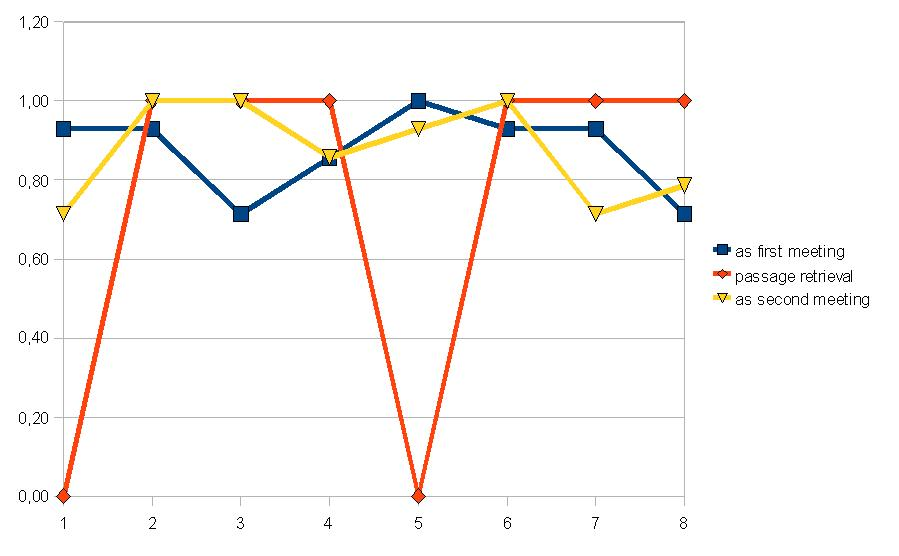
\includegraphics[width=1\textwidth]{BET_results_compararison_IB4010_passage.jpg}
%%\caption{Compararison with BET results for IS1008c (Passage retrieval)}
%\end{minipage}
%\hfill
%\begin{minipage}{5cm}
%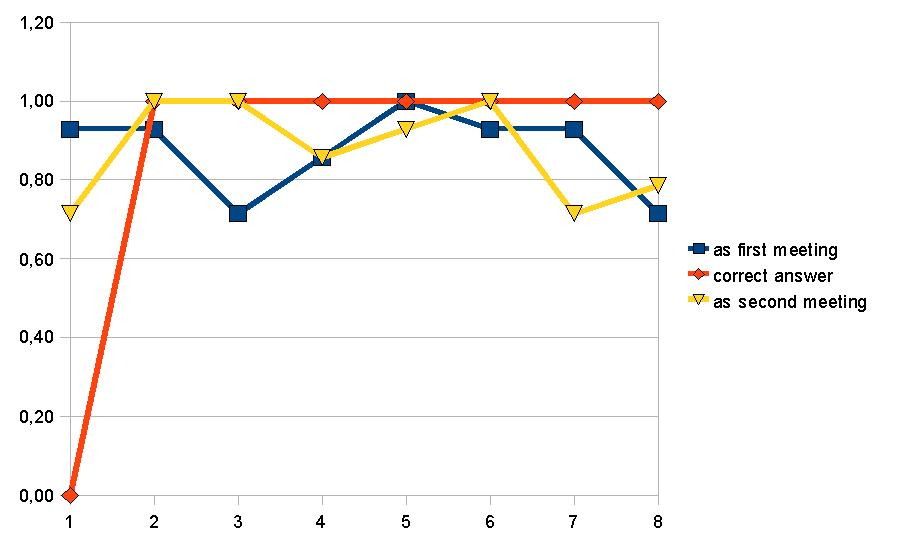
\includegraphics[width=1\textwidth]{BET_results_compararison_IB4010_truefalse.jpg}
%%\caption{Compararison with BET results for IS1008c (True-false questions answering}
%\end{minipage}
%\caption{Comparison with BET results for IB4010}
%\end{figure}
 




%Say that they come from previous study + reference

%Chu thich nguon du lieu tu BET, quota the paper on BET4TQB

According to the BET for TQB \cite{popescubelis2007otm}, average precision to answer all BET questions for IB4010 is 0.85 \ensuremath{\pm} 0.05 and 0.70 \ensuremath{\pm} 0.10 for IS1008c. For human subjects, we can divide the BET questions into two groups: \textit{easy} and \textit{difficult}. A BET question belongs to the \textit{easy} group  if average precision of its answers as first meeting or second meeting is more than 0.85 for IB4010 and 0.70 for IS1008c, otherwise it belongs to the \textit{difficult} group. Meanwhile, for the system, the \textit{easy} group includes all questions that  their number of correct passage or number of correct true-false answer is 1.
This help us have a standard to compare the BET scores by humans with scores obtainned by the system.

We first examine the results for IB4010. According to the convention above, for human subjects there is only one \textit{difficult} question (question number 8), while there are two \textit{difficult} questions for the system (questions number 1 and 5). In fact, all of these questions are \textit{deductive questions} that require deep comprehension rather than a search of lexical similarities. For the question number 1, the true and the false statement in this pair are \textit{The group decided to show The Big Lebowski} and \textit{The group decided to show Saving Private Ryan} respectively. This question requires to read all of the transcript before answering the question. That is why the system could not identify the correct passage using a small search window that does not cover all the information of the transcript as it requires for this type of question. Consequently, the true-false answer is determined by chance (false in this case). The question number 5 also requires a deduction to distinguish the true statement \textit{No one had seen Goodfellas} from the false statement \textit{Everyone  had seen Goodfellas}. In the meeting, when all meeting participants said \textit{No} for the question \textit{Have you seen Goodfellas?}, it is easy for human subjects to understand the answer of the participants. However, this is really a difficult task for an automatic system.  The system identified the incorrect passage. Consequently, its true-false answer is determined by chance, that is true in this case. Question number 8, whose the true and the false statement are \textit{Agnes eliminates Pulp Fiction as she dislikes Quentin Tarantino} and \textit{Agnes eliminates Pulp Fiction as it is too violent} is also a deductive question because it is not easy to match the question \textit{I dislike Quentin} with the text \textit{I am not a huge fan of Quentin Tarantino}. However, the system gave the true answer for this question while it was difficult for human subjects. That is because the keyword Quentin appears only one time in the transcript and the system was based on this word, but not based on the meaning of the essential phrase to identify the correct passage.

\begin{table}[ht!]
\scriptsize
\caption{Comparison with BET scores by human subjects for IS1008c}
\begin{tabular}{|c|r|r|r|r|r|r|r|}
\hline
\multicolumn{ 1}{|c|}{curQuid} & \multicolumn{ 4}{c|}{Humans} & \multicolumn{ 3}{c|}{System} \\ \cline{ 2- 8}
\multicolumn{ 1}{|l|}{} & \multicolumn{1}{c|}{Precis1} & \multicolumn{1}{c|}{avg time1} & \multicolumn{1}{c|}{Precis2} & \multicolumn{1}{c|}{avg time2} & \multicolumn{1}{c|}{\#cpassage} & \multicolumn{1}{c|}{\#canswer} & \multicolumn{1}{c|}{\#time} \\ \hline
1 & 0.86 & 410 & 0.93 & 127.36 & 1 & 1 & 13 \\ \hline
2 & 0.67 & 298.58 & 0.86 & 129.5 & 1 & 1 & 45 \\ \hline
3 & 0.82 & 78.09 & 0.93 & 67.5 & 1 & 1 & 15 \\ \hline
4 & 0.89 & 80.22 & 0.93 & 103.93 & 1 & 1 & 16 \\ \hline
5 & 0.63 & 66.38 & 0.69 & 63.92 & 1 & 0 & 20 \\ \hline
6 & 0.67 & 44 & 0.73 & 62.18 & 0 & 0 & 10 \\ \hline
7 & 1.00 & 24 & 0.82 & 48 & 1 & 0 & 11 \\ \hline
8 & 0.67 & 66 & 0.64 & 93.55 & 0 & 1 & 11 \\ \hline
\multicolumn{1}{|l|}{} & \textbf{0.77} & \textbf{133.41} & \textbf{0.81} & \textbf{86.99} & \textbf{0.75} & \textbf{0.63} & \textbf{17.63} \\ \hline
\end{tabular}
\label{table: BET scores for IS1008c}
\end{table}

For IS1008c, as defined above, for \textit{easy} and \textit{difficult} questions there are two \textit{difficult} questions for human subjects. They are questions numbered 5 and 8. For the system, it incorrectly answered three questions that are questions numbered 5, 6,7 and 8, in which the questions numbered 5, 6 and 8 are deductive questions. For question numbered 5, whose the true statement is \textit{Agnes express her opinion that ...}, the correct passage should be \textit{Agnes: I think ... }. Two different expressions make it difficult to understand for both human subjects and the automatic system. With regard to question number 6, whose the true statement is \textit{Agnes notes some reasons to not have a display} and the false statement is \textit{Agnes tries to persuade the group they should have a display}, Agnes showed a list of reasons in the transcript but there is few matched words between question string and answer string. This is similar with question number 8, which has the true statement and the false statement are \textit{Market research suggests the remote has to be new and different.} and \textit{Market research suggests the remote has to be comfortable and familiar.} respectively. However, the true-false answer for question numbered 8 is correct by chance. Question number 7 is not difficult. It has the true statement and the false statement are \textit{Ed commented that they had a product but that cost was going to be a potential problem} and \textit{Ed commented that they had a product and that cost was not going to be a problem} respectively. For this question the system gave correct passage but incorrect true-false answer. That means true-false answers by the system are not as stable as correct passage answering.

In conclusion, although both human subjects and the system encounter difficulties to answer deductive questions, these are more difficult for the automatic system. For IB4010, there are 3 deductive questions and the automatic system incorrectly answered 2 out of 3 questions, while at the same time, the human subjects have difficulty only answering 1 of the 3 questions. For IS1008c, there are also 3 deductive questions. The system gave the wrong answers for all three questions, meanwhile the human subjects had difficulty answering two questions. In fact, deductive questions are equivalent to How and Why questions that are difficult for all question answering systems \cite{prager2000qap, brill2002diq}.

According to the experimental results, the results for the passage retrieval are more logical than the results for true-false answers. That means the system should be developed to help humans answer BET-typed questions by identifying relevant passage instead of giving the final answers. In other words, it is a useful tool for locating the answer, but not necessarily for answering questions directly \cite{lequocanh1}.
 

\newpage




